\chapter{Modelo Conceitual}

Este capítulo apresenta um modelo de utilização de \textit{templates} multicamadas para construir e manipular questões de programação. A ideia inclui o emprego de inteligência artificial generativa como ferramenta complementar, responsável por sugerir variações criativas no \textit{template} base, tais como modificações de contexto, acréscimo de novos cenários e introdução de pontos de variação. Além disso, a IA generativa também oferece suporte no fornecimento de \textit{feedback} imediato ao estudante após a submissão da resposta, apontando erros, sugerindo melhorias e apresentando explicações detalhadas sobre o problema e possíveis soluções. 

\section{Geral para o Específico}
A geração automática de questões segue um processo hierárquico que se inicia em tópicos mais amplos e evolui até questões específicas. Em primeiro lugar, são definidos os tópicos da ementa, que correspondem a áreas ou domínios do conhecimento a serem avaliados (por exemplo, Estruturas de Repetição, Estruturas de Decisão, Matrizes, Funções). Esses tópicos abrangem conteúdos específicos do currículo e orientam a elaboração dos modelos cognitivos. Na etapa seguinte, estes modelos cognitivos são convertidos em \textit{templates}, que servirão de base para a geração das questões. Essa abordagem reflete a metodologia recomendada para a criação de questões baseadas em \textit{templates}. 

\begin{figure}[ht]
	\centering
	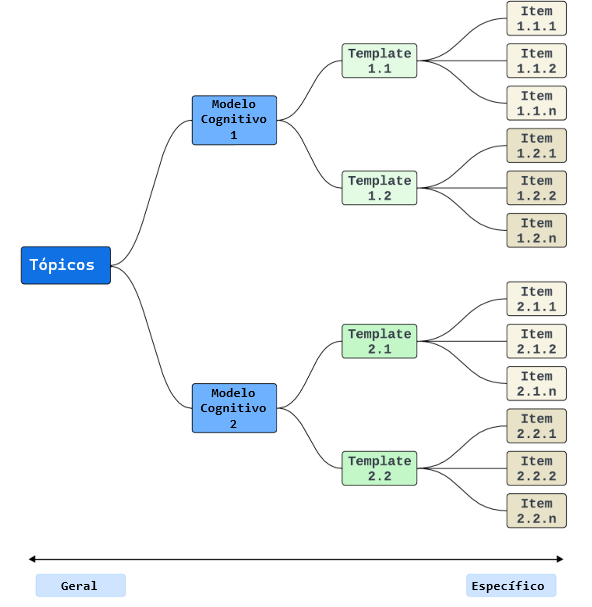
\includegraphics[width=14cm]{./imagens/capitulo5/geral-especifico-com-topicos}
	\caption{Geral para o específico, (Adaptado, \cite{hendrickson2010}) }
	\label{fig:geral-to-specif}
\end{figure}


\section{Escala de proficiência}

A classificação das questões com base em atributos e características, como o nível de dificuldade, é essencial nas avaliações educacionais. Agrupar questões por níveis de dificuldade (fácil, médio e difícil) possibilita organizar bancos de questões que atendem diferentes perfis de estudantes.  Esse agrupamento é especialmente relevante em contextos que utilizam testes adaptativos, onde o sistema ajusta a dificuldade das questões apresentadas de acordo com o nível de aptidão do aluno. Assim, é possível proporcionar uma experiência de aprendizado personalizada, onde cada questão apresentada se adequam ao desempenho e à evolução do aluno ao longo das avaliações \parencite{pasquali2018}. A figura \ref{fig:proficiency-scale}  ilustra um banco de modelos estruturado para oferecer templates compatíveis com diferentes níveis de dificuldade. Esse tipo de organização permite um maior controle sobre a dificuldade das questões geradas.


\begin{figure}[ht]
	\centering
	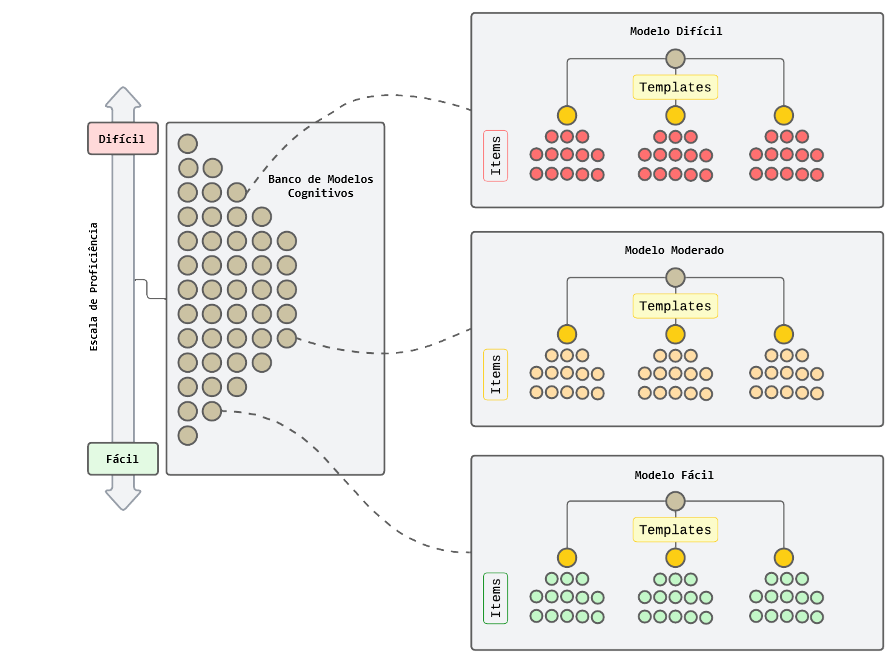
\includegraphics[width=14cm]{./imagens/capitulo5/proficiency-scale-named}
	\caption{Geral para o específico, (Adaptado, \cite{hendrickson2010}) }
	\label{fig:proficiency-scale}
\end{figure}

\section{Estrutura dos Templates em JSON}

O JSON foi adotado como formato padrão para a construção dos templates de questões devido ao seu alto desempenho, simplicidade e facilidade de uso. Em comparação ao XML, o JSON mostrou mais eficiente em diversas métricas, conforme demonstrado no trabalho de \parencite{wang2011}, que indica um ganho de  48,56\% na velocidade de carregamento de 1000 objetos por página comparado com o XML. Esse resultado deve, em grande parte, à estrutura mais enxuta do JSON, que demanda menos esforço de interpretação se comparado ao uso extensivo de \textit{tags} no XML.  Além disso, o JSON oferece suporte nativo a tipos de dados como \textit{arrays}, números, \textit{strings} e valores booleanos, o que simplifica o tratamento de estruturas hierárquicas — característica fundamental na representação de templates de questões.

\begin{figure}[ht]
	\centering
	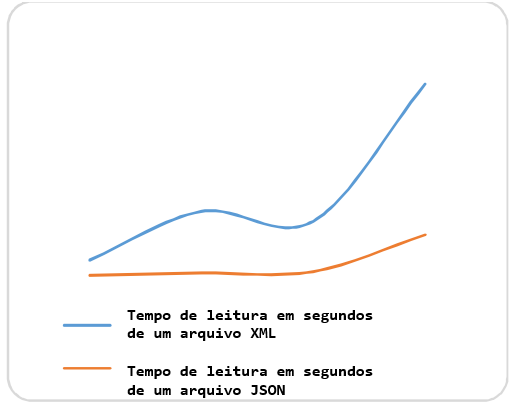
\includegraphics[width=10cm]{./imagens/capitulo5/json-vs-xml}
	\caption{Comparação de leitura JSON vs XML, \parencite{goyal2017} }
	\label{fig:json-vs-xml}
\end{figure}

Outro fator relevante é a compatibilidade do JSON com linguagens modernas, como JavaScript, Python e Java, eliminando a necessidade de bibliotecas externas para análise (\textit{parsing}) ou manipulação de dados. Já o XML frequentemente exige mais recursos para tratamento de \textit{tags} e maior esforço de processamento. A análise de desempenho citado por \parencite{goyal2017} destaca que o JSON, por ser mais leve e simples, tem melhor tempo de leitura em aplicações com pares de chave-valor, conforme a figura \ref{fig:json-vs-xml}. Assim, sua adoção torna o desenvolvimento de sistemas mais eficiente e escalável, justificando sua escolha como formato preferencial para os templates de questões neste trabalho.


\section{Representação Hierárquica dos Templates em JSON}

Inicialmente, escrever o modelo de questão em um editor de texto é uma prática útil para planejar a estrutura do template. No entanto, a fase seguinte envolve a estruturação desse modelo em formato JSON, o que facilita a manipulação e a geração de questões de forma automatizada. A transição para JSON permite que o template seja editado e gerenciado, permitindo o desenvolvimento de \textit{scripts} ou algoritmos capazes de gerar automaticamente diversas instâncias de questões a partir do template.
A Figura \ref{fig:template-json-example-1} descreve como o template pode ser organizado no formato JSON, que é composto por três componentes : Texto Principal (\textit{Stem}), Variáveis e as Multicamadas (\textit{N-Layers}). Cada elemento desempenha um papel específico conforme as seguintes finalidades:


\begin{itemize} \item \textbf{Texto Principal (\textit{Stem})} \begin{itemize} \item Representa o texto base da questão, servindo de ponto de partida para a formulação do template. Nele contém trechos fixos e indicações de onde as variáveis serão inseridas, tornando a questão adaptável a diferentes contextos. \end{itemize}
\item \textbf{Variáveis (\textit{Variables})}
\begin{itemize}
    \item Inclui parâmetros e conteúdos  que podem variar, permitindo a personalização do texto principal com indicações de onde serão inseridas no enunciado, de forma que permita a flexibilidade e reutilização destas variáveis em outros cenários específicos.
\end{itemize}

\item \textbf{Multicamadas (\textit{N-Layers})}
\begin{itemize}
    \item Funcionam como \textit{subtemplates} dentro do template principal, que possibilita a inclusão de novas variáveis e conteúdos para expandir e adaptar o enunciado da questão em diferentes cenários, um sub-template sempre deriva do template principal.
    \end{itemize}
\end{itemize}


\begin{figure}[ht]
	\centering
	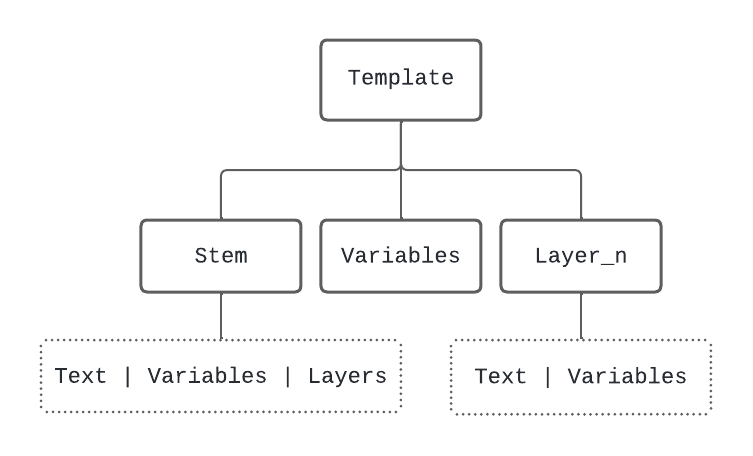
\includegraphics[width=14cm]{./imagens/capitulo5/template-json-example-1}
	\caption{Estrutura do template de questões (Elaboração própria, 2025) }
	\label{fig:template-json-example-1}
\end{figure}


\section{Mecanismo de Combinação}

O mecanismo de combinação consiste em um processo de geração de questões a partir do \textit{template} principal, descrito no formato JSON, que contém estruturas de texto e múltiplas opções de conteúdo. Esse \textit{template} atua como um conjunto de possibilidades, permitindo que novas perguntas sejam criadas de forma sistemática, por meio da seleção e combinação das variações de cada campo.

Para que o \textit{template} seja aplicado em diferentes cenários, é utilizado um segundo arquivo JSON onde cada chave representa a configuração de uma questão específica e cada valor corresponde ao índice selecionado em cada campo do \textit{template}. Dessa forma, se no campo \textbf{"introducao": ["intro\_1", intro\_2", "intro\_3"]} caso a questão for exigido a segunda opção, o valor referenciado será o índice \texttt{\textbf{1}} (assumindo zero como base de indexação). Essa abordagem sistematiza a produção automatizada de questões, pois basta apenas alterar os índices para gerar combinações distintas, sem alterar a estrutura original do texto.

A Figura \ref{fig:template-1} (referente ao \textit{template}) e a Figura \ref{fig:template-2} (referente às instâncias de questões) apresentam esse processo. Enquanto a primeira foca nos template em si e seus valores possíveis, a segunda demonstra como cada questão seleciona um conjunto de índices para formar a questão final. 

\begin{figure}[ht]
	\centering
	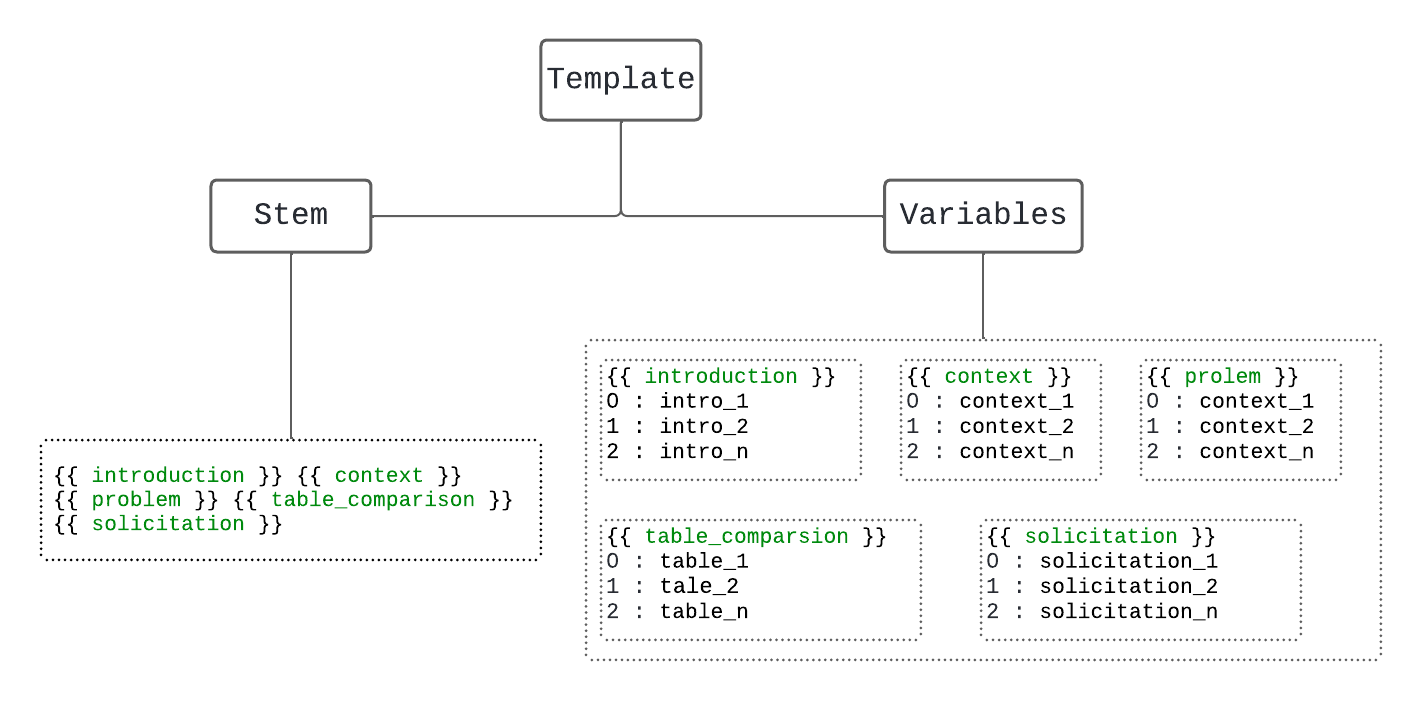
\includegraphics[width=16cm]{./imagens/capitulo5/template-1}
	\caption{JSON : Template principal (Elaboração própria, 2025) }
	\label{fig:template-1}
\end{figure}

\begin{figure}[ht]
	\centering
	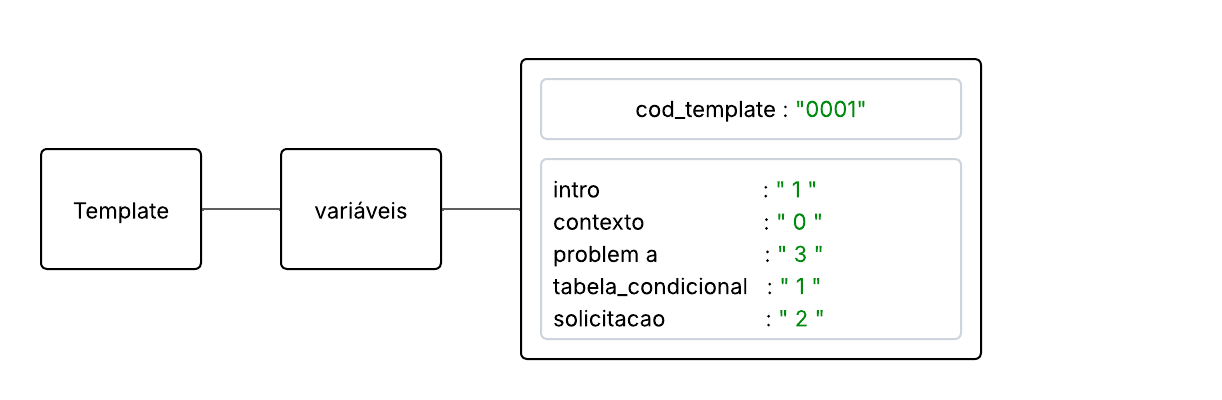
\includegraphics[width=18cm]{./imagens/capitulo5/template-2}
	\caption{Template de questões (Elaboração própria, 2025) }
	\label{fig:template-2}
\end{figure}

\section{Algoritmos Utilizados}

Nesta seção será apresentado os algoritmos empregados para gerar as questões de forma automática a partir de dois arquivos JSON distintos: um contendo o template (JSON de Template), e outro contendo as questões (JSON de Questões). O \textit{JSON de Template} reúne a estrutura de cada parte de uma questão e as possíveis variações de conteúdo que podem ser combinadas. Já o \textit{JSON de Questões} consiste em um conjunto de chaves que apontam para índices específicos dentro das listas de opções do \textit{JSON Template}, permitindo a criação de múltiplas versões a partir de um único template. 
Para a construção das questões, foram definidas duas funções principais, descritas nos Algoritmos \ref{alg:generate_questions} e \ref{alg:get_feedback}  respectivamente.   
O primeiro algoritmo percorre os índices listados no \textit{JSON de Questões} e combina cada referência com o campo do \textit{JSON de Template}, devolvendo todas as questões geradas.  
A segunda função, apresentada no Algoritmo \ref{alg:get_feedback}, recebe o enunciado produzido e o codigo submetido pelo usuário e, com auxlio de um modelo de \gls{llm} (especificamente o GPT-4), interpreta o problema, avalia a solução, identifica inconsistências e sugere uma versão corrigida com feedback detalhado. Essa integração de IA reduz significativamente o custo de validação manual.

\begin{algorithm}[H]
\caption{Geração de Questões Multicamadas}
\label{alg:generate_questions}
\KwIn{\textbf{Template}, \textbf{TemplateQuestões}, \textbf{QtdItens} (opcional), \textbf{SelectOne} (opcional)}
\KwOut{Lista de questões geradas ou uma única questão, conforme o parâmetro \textbf{SelectOne}}

Carregar o objeto \textbf{Template} a partir de \textit{templatePath}\;
Carregar o objeto \textbf{TemplateQuestões} a partir de \textit{questionPath}\;

\If{\textbf{Template.codTemplate} $\neq$ \textbf{TemplateQuestões.codTemplate}}{
    \Return Erro: códigos de template incompatíveis\;
}

Definir \textbf{Qtd} $\gets$ número de itens a gerar, respeitando o total disponível\;
Inicializar a lista \textbf{QuestõesGeradas} como vazia\;

\For{cada elemento $q$ em \textbf{TemplateQuestões.questoes}, até o limite \textbf{Qtd}}{
    Definir \textbf{CabecalhoPrincipal} $\gets$ \textbf{Template.stem}\;

    \If{existe camada \textbf{layer-1} em \textbf{Template} \textbf{e} variáveis de camada em $q$}{
        Processar as variáveis da camada \textbf{layer-1}\;
        Substituir os placeholders da camada no \textbf{CabecalhoPrincipal}\;
    }

    Substituir as variáveis de \textbf{CabecalhoPrincipal} com base em \textbf{cabecalho-var} de $q$\;
    Adicionar \textbf{CabecalhoPrincipal} à lista \textbf{QuestõesGeradas}\;
}

\If{\textbf{SelectOne} é verdadeiro}{
    \Return Uma questão aleatória de \textbf{QuestõesGeradas}\;
}
\Else{
    \Return A lista completa \textbf{QuestõesGeradas}\;
}
\end{algorithm}





\begin{algorithm}[H]
\caption{Geração de Feedback Automatizado para Submissões de Código}
\label{alg:get_feedback}
\KwIn{\textbf{EnunciadoQuestao}, \textbf{CodigoSubmetido}, \textbf{ChaveAPI}}
\KwOut{Texto com feedback detalhado sobre a submissão}

Inicializar o cliente da API \textbf{OpenAI} utilizando \textbf{ChaveAPI}\;

Definir a lista de mensagens \textbf{Mensagens} com o seguinte conteúdo:\;
\Indp
\textbf{(i)} Um prompt de sistema informando que o modelo atua como revisor de código\;
\textbf{(ii)} Uma mensagem de usuário contendo o enunciado da questão, o código submetido e as instruções para correção e feedback\;
\Indm

Tentar gerar a resposta com os seguintes parâmetros:\;
\Indp
\textbf{Modelo}: \textit{GPT-4}\;
\textbf{Aleatoriedade}: $1$\;
\textbf{Máximo de Tokens}: $1000$\;
\textbf{Mensagens}: \textbf{Mensagens}\;
\Indm

\If{a geração for bem-sucedida}{
    Retornar o conteúdo textual da resposta do modelo\;
}
\Else{
    Capturar a exceção e retornar uma mensagem de erro descritiva\;
}
\end{algorithm}




 
\section{Fluxo de Trabalho}


O fluxo de trabalho representado pelo \gls{bpmn} da Figura \ref{fig:bpmn-fluxo} coordena de modo colaborativo as interações entre o professor (\emph{especialista}), o \textbf{sistema}, dois \textbf{serviços de IA} e o \textbf{aluno} no contexto da geração automática de questões. Seu propósito é apoiar a criação e a validação das questões geradas a partir de \textit{templates} e oferecer \textit{feedback} das respostas submetidas pelos estudantes.

\textbf{Papel do especialista.} O processo inicia com o professor, que \emph{define o modelo cognitivo} e \emph{elabora os templates} das questões. Em seguida, valida os pontos de variação desses templates, assegurando que as versões propostas pela IA estejam alinhadas com os objetivos pedagógicos.

\textbf{Papel do sistema e dos serviços de IA.} Uma vez validados, os templates alimentam o sistema, que os disponibiliza aos estudantes e aciona dois serviços externos de IA:

\begin{itemize}
\item \textbf{Sugestão de Variações} – gera automaticamente novas instâncias de questões com base nos pontos de variação definidos pelo professor, ampliando a diversidade de cenários.
\item \textbf{Geração de Feedback} – analisa as respostas dos alunos, identifica erros ou inconsistências e produz orientações de como responder o enunciado corretamente.
\end{itemize}

\textbf{Papel do aluno.} O aluno é o principal beneficiado desse fluxo. Ele \emph{visualiza} as questões geradas, \emph{envia} suas respostas e por fim \emph{recebe} feedback sobre a submissão do código, o que contribui para a identificação de erros, a correção de conceitos e consequentemente, para a melhoria contínua de seus conhecimentos.

\begin{figure}[ht]
\centering
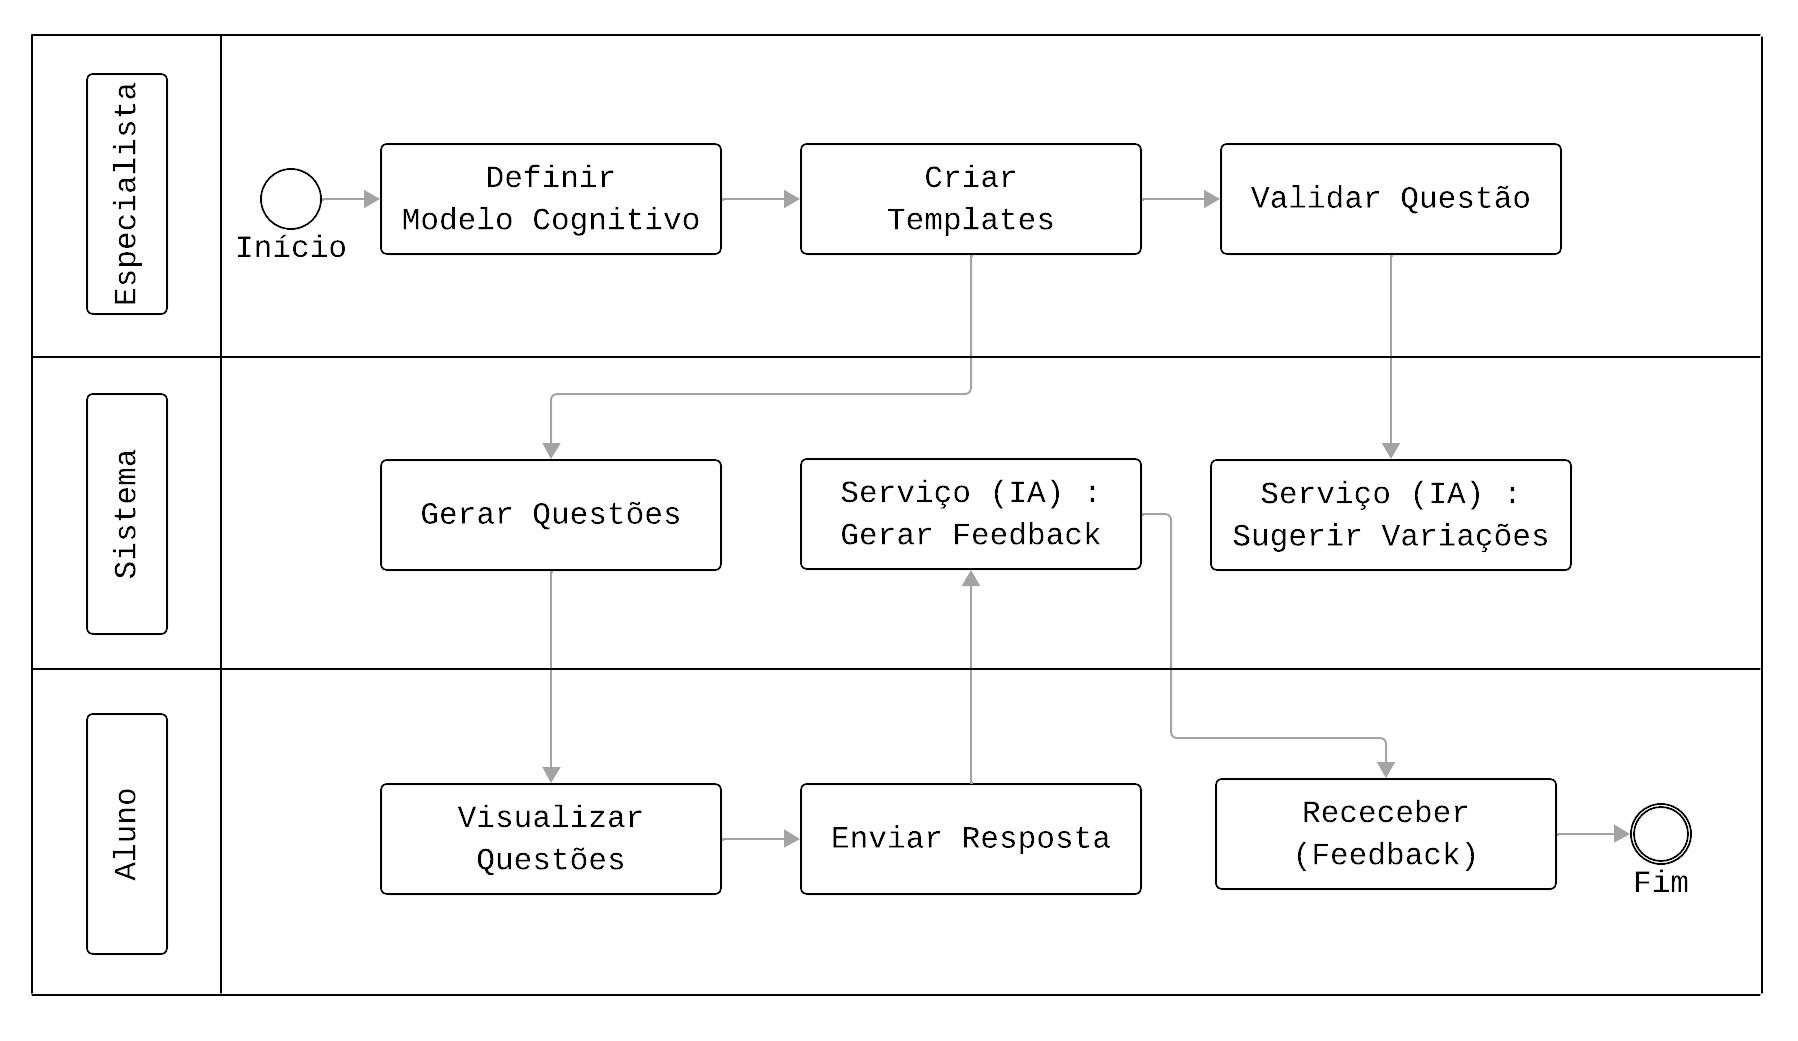
\includegraphics[width=16cm]{./imagens/capitulo6/bpmn-fluxo}
\caption{BPMN do fluxo de trabalho (elaboração própria, 2025).}
\label{fig:bpmn-fluxo}
\end{figure}

\bigskip
\noindent


Tendo estabelecido os fundamentos teóricos e a dinâmica de interação descritos neste capítulo, o capítulo seguinte apresentará a implementação do sistema. Serão detalhadas suas principais interfaces e uma análise dos benefícios e limitações da abordagem proposta.